\documentclass{article}
\usepackage{url,graphicx,color,hyperref}
\newcommand\anote[2]{{\color{#1}\bf #2}}
\newcommand\anil[1]{{\anote{red}{anil: #1}}}


\begin{document}

\title{MUSINGS: Walking the Type Rope: from Idris to OCaml to machine code}
\author{Anil Madhavapeddy etc}

\maketitle

\section{Introduction}

Working with precise wire formats in high-level languages is difficult to do in an efficient way.
Internet formats in particular are quite variable---low-level bit-wise parsing for IP stacks, ABNF parsing for common protocols such as HTTP or IMAP, tree-parsers for XML or JSON, and cryptographic and compression layers with SSL and zlib.
The complexity is further compounded by the fact that applications need to sequentially apply these different parsers to incoming data, as well as {\em generate} new responses.

Currently, a common strategy in high-level languages is to copy the results of a parse stages into separate buffers. This incurs a big performance penalty, as well as drives up garbage collection pressure.
Another big performance loss is bounds checking buffer accesses in each parser stage, rather than amortising all the checks in one go.
Finally, the {\em programmer interfaces} for constructing and parsing packets tends to be very inconsistent---although there are quite a few parser generators available, none of them provide rich enough name bindings to permit packet constructors to also be generated from the same specification.

Our overall goal is to create an efficient (zero-copy) API to handle I/O across a variety of protocols, without the programmer having to worry about the low-level wire details\footnote{These ``low-level wire details'' are also the source of hundreds of millions of dollars worth of security bugs in some of the most popular servers on the Net...}.  It would be very nice if it could also work with multiple languages---we start with a series of protocol descriptions, and end up with an appropriate interface for target language (e.g. a type in Idris, a C library, or an OCaml module)

In this document, we describe {\em Type Ropes}: a system for handling incoming streams of data, zero-copy parsing them into high-level data structures, and providing strongly typed interfaces to construct responses.  Type ropes entirely replace conventional I/O interfaces such as buffered channels with strongly typed equivalents that guarantee that a server can never emit invalid protocol responses.  They also free the programmer from having to worry about concrete data representations entirely, and focus on the protocol state machine.

\section{Describing Protocols}

All parsers are defined  as a series of Domain Specific Languages that suit the language at hand.

\subsection{MPL}

MPL is for defining low-level binary formats, as seen in Internet protocols such as IP, TCP, BGP, Ethernet, DNS or DHCP\footnote{See \url{http://anil.recoil.org/papers/2007-eurosys-melange.pdf}}. Lots of MPL specifications are available at \url{http://github.com/avsm/mirage/tree/master/lib/mpl}.  There are also the associated auto-generated OCaml interfaces in that directory.

\subsection{ABNF}

ABNF grammars are useful for many textual Internet protocols, such as HTTP, SMTP or IMAP.  Unfortunately, the RFCs that specify them are very inconsistent, often making up ABNF terminology and reverting to informal language to describe a portion of the parse.

An ABNF specification parser is available on Github\footnote{\url{http://github.com/avsm/ocaml-abnf}} along with the large ABNF specifications for HTTP and IMAP\footnote{\url{http://github.com/avsm/ocaml-abnf/tree/master/imap.abnf}}.  Almost every HTTP and IMAP implementation in existence seems to be hand-crafted rather than using an autogenerated grammar such as these, for some reason.

{\em Note:} the ABNF specifications here are still a work-in-progress: they do not have sufficient name bindings in the DSL to generate nice packet constructors at present.

\subsection{JSON, XML, etc}

There are several schema generators for XML and JSON available that map the underlying tree structures onto strongly typed values, but with in inconsistent interfaces (using an input string or buffered I/O channel).

\subsection{Using these DSLs}

These DSLs contain sufficient information to auto-generate language code that will parse raw buffers of that data into a higher level language structure.  Next, we will discuss what a common buffer representation for these would look like, and then discuss how this code might actually be generated.

\section{A Buffer Representation}

Now that the wire formats are described sufficiently that typed interfaces can be generated for them, we need to consider how to implement them.

The simplest and most efficient way (multicore considerations aside for the moment) to handle I/O is as a stream of frames. Operating systems typically implement buffered I/O on top of this, but this causes more unnecessary data copying.  We assume that the language also provides a lightweight threading system to handle blocking (but not necessarily preemptive).

\begin{figure}
\centering
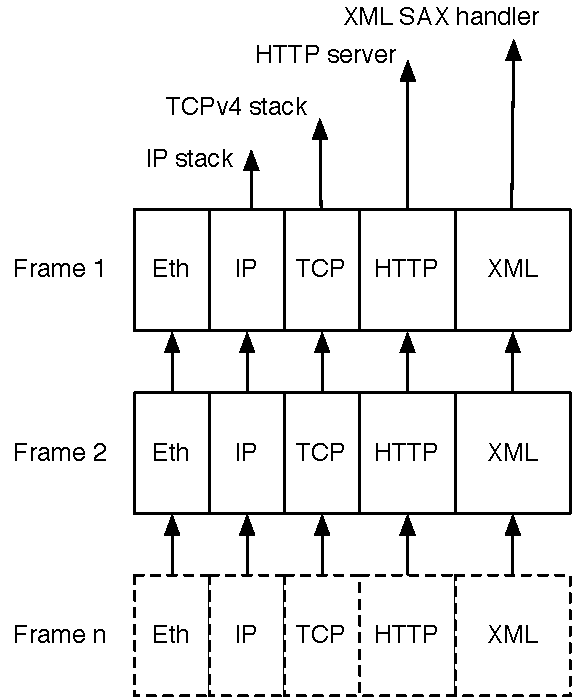
\includegraphics[height=8cm]{ropes.pdf}
\caption{\label{fig:ropes}A series of incoming buffers being classified into type ropes}
\end{figure}

Figure~\ref{fig:ropes} illustrates the buffer setup for an Ethernet stack (but the same principles apply if using, for example, POSIX sockets).  Incoming data is read in as frames (a set of unparsed bytes).  The frame is immutable, and is classified by the DSLs in the previous section.

As each parser finishes classifying, it constructs a smaller sub-view of the buffer and passes that to the next parser in the chain. If it requires more data to complete the parse, it will block using a lightweight thread. 
Eventually, the application can retrieve values from this buffer using the types generated from the DSL.

Packet construction works in a slightly different way: applications must build up their responses as a series of closures (similar to a monad signature, but not quite)\footnote{See \url{http://anil.recoil.org/papers/2007-eurosys-melange.pdf} for a longer explanation if this doesn't make any sense.}.  The DSL code then applies these in sequence, while also inserting automatic fields such as packet lengths or checksums to the buffer.   If the parser runs out of buffer space in any of the layers (e.g. IP fragmentation), it blocks until a new output frame is available.

\subsection{An aside: intermediate buffer language}

There are some operations on buffers which are very commonly needed by parsers, and for which very fast assembly language instructions are available (or vector intrinsics in some cases).  When parser generators go via C, they lose a lot of this type information to optimise the binary output.  Speed matters in the data plane, though!

For example, on {\tt x86}, an instruction called {\tt SCASB} can scan a fixed-size string for a specific byte with a single instructions (this is how {\tt strlen} is usually implemented in {\tt libc}).  Thus, tasks like ``scan for newline'' for variable-length grammers (as seen in ABNF or XML) could be immensely sped up as opposed to scanning byte-by-byte.

So, it would be nice to compile down the DSLs into an intermediate set of parser opcodes that could be directly output as assembly parse instructions instead of hopping through C/GCC.


\section{Implementing these DSLs}

Currently, the MPL and ABNF spec compilers read in a specification and output OCaml code as a manually implemented compiler.  However, this is a really nice potential use case for partial evaluation: 

\begin{itemize}
\item Begin with a specification interpreter (MPL, ABNF, XML, etc), and hand it a concrete specification.
\item Partially evaluate this down to a parsing intermediate language
\item Generate the typed interface for construction/deconstruction of the protocol.
\item If target language is Idris, continue to implement the full server state machine.
\item If target language is a less rich type system (e.g. OCaml), then stringify the typed output into a concrete OCaml module.
\item For all languages, the parsing intermediate language can be converted to LLVM or direct x86 output (or just interpreted, for debugging use initially).
\end{itemize}

If it works, it gives us a nice framework to not have to worry about pesky wire formats again! If some new wire format comes up that doesnt fit into any of these (e.g. DNS labels), it can just be implemented in Idris as an EDSL, but reuse all the rest of the scaffolding.
Above all, having a unified way of handling data would be a huge leap in constructing network servers... 

\end{document}